% 07-hieu-qua.tex — Chương 7: Hiệu quả, lợi ích và chỉ tiêu đo lường

\chapter{Hiệu quả, lợi ích và chỉ tiêu đo lường}\label{ch:hieuqua}

\begin{tomtat}[Cách tiếp cận]
Hiệu quả kinh doanh của một hệ thống dự báo \textbf{không thể suy ra chỉ từ độ chính xác của mô hình}. Chương này trình bày
(1) lợi ích kỳ vọng, (2) cách lượng hóa giá trị, (3) bộ chỉ tiêu đo lường đề xuất và (4) thiết kế thử nghiệm đối chứng để chứng minh hiệu quả bằng số liệu thực tế.
\end{tomtat}

\section{Lợi ích trực tiếp}

{\tablefont
\begin{longtable}{@{}>{\bfseries}L{3.8cm}>{\raggedright\arraybackslash}p{11.83cm}@{}}
\caption{Lợi ích trực tiếp của sáng kiến}\label{tab:loiich}\\
\toprule
\hdrrow\hh{Lợi ích} & \hh{Diễn giải}\\
\midrule
\endfirsthead
\toprule
\hdrrow\hh{Lợi ích} & \hh{Diễn giải}\\
\midrule
\endhead
\bottomrule
\endfoot
Phát hiện sớm & Cảnh báo trước 1--2 tháng, khi vẫn còn cơ hội can thiệp, thay vì phát hiện sau khi khách đã chuyển sang đơn vị khác.\\
\rowa Tập trung nguồn lực & Thay vì chăm sóc dàn trải, đội chăm sóc ưu tiên nhóm 5\% rủi ro cao nhất; thời gian chăm sóc được đặt vào nơi có khả năng tạo giá trị cao nhất.\\
Hành động đúng nguyên nhân & Lý do rủi ro cho biết nên xử lý khiếu nại, cải thiện chất lượng khai thác hay chăm sóc chủ động.\\
\rowa Tiết kiệm công sức tổng hợp & Dữ liệu, chỉ số, chấm điểm và xuất danh sách chạy tự động; cán bộ không phải tổng hợp thủ công nhiều nguồn.\\
Số liệu nhất quán & Một nguồn dữ liệu, một bộ công thức cho mọi báo cáo; hạn chế mâu thuẫn do các đơn vị tự tổng hợp.\\
\rowa Chất lượng được kiểm soát & Cổng xét duyệt mô hình và giám sát độ lệch giúp kết quả đáng tin cậy theo thời gian.\\
\end{longtable}}
\vspace{4pt}

\section{Lợi ích dài hạn}

\begin{itemize}
  \item \textbf{Tích lũy tài sản dữ liệu:} mỗi kỳ chấm điểm tạo thêm lịch sử rủi ro của từng khách hàng, phục vụ phân tích xu hướng theo nhiều tháng.
  \item \textbf{Vòng phản hồi:} kết quả chăm sóc được ghi nhận quay lại làm nhãn thực tế, giúp mô hình ngày càng sát nghiệp vụ.
  \item \textbf{Hiểu nguyên nhân rời bỏ:} thống kê lý do rủi ro theo vùng, dịch vụ, nhóm khách giúp lãnh đạo nhận diện điểm yếu của chất lượng dịch vụ và chính sách, không chỉ xử lý từng khách.
  \item \textbf{Nền tảng cho các bài toán tiếp theo:} cùng dây chuyền dữ liệu có thể dùng cho phân khúc khách hàng, tối ưu ngân sách chăm sóc (Chương~\ref{ch:morong}).
\end{itemize}

\section{Cách lượng hóa giá trị kinh doanh}

Giá trị tạo ra của hệ thống nên được tính bằng công thức đơn giản, mọi biến số đều có thể lấy từ dữ liệu thực tế sau thử nghiệm:

\begin{center}
\begin{callout}{lightgray}{black}{}
\sffamily\small\sffamily
\textbf{Giá trị giữ lại} = (Tỷ lệ khách giữ lại nhóm áp dụng $-$ Tỷ lệ khách giữ lại nhóm đối chứng)\\
$\times$ Số khách được can thiệp $\times$ Doanh thu bình quân mỗi khách trong kỳ\\[4pt]
\textbf{Hiệu quả ròng} = Giá trị giữ lại $-$ Chi phí hệ thống $-$ Chi phí chăm sóc phát sinh
\end{callout}
\end{center}

{\tablefont
\begin{longtable}{@{}L{5.6cm}C{3.2cm}>{\raggedright\arraybackslash}p{6.41cm}@{}}
\caption{Các biến cần điền sau thử nghiệm}\label{tab:bienso}\\
\toprule
\hdrrow\hh{Biến số} & \hh{Giá trị} & \hh{Nguồn lấy số liệu}\\
\midrule
\endfirsthead
\toprule
\hdrrow\hh{Biến số} & \hh{Giá trị} & \hh{Nguồn lấy số liệu}\\
\midrule
\endhead
\bottomrule
\endfoot
Số khách được can thiệp (nhóm áp dụng) & \phc{~} & Danh sách top 5\% và nhật ký chăm sóc\\
\rowa Tỷ lệ giữ lại nhóm áp dụng & \phc{~\%} & Đơn hàng sau 1--2 tháng\\
Tỷ lệ giữ lại nhóm đối chứng & \phc{~\%} & Đơn hàng sau 1--2 tháng\\
\rowa Doanh thu bình quân mỗi khách/kỳ & \phc{~} & Dữ liệu doanh thu\\
Chi phí chăm sóc phát sinh & \phc{~} & Đơn vị chăm sóc khách hàng\\
\end{longtable}}
\vspace{4pt}

\section{Bộ chỉ tiêu đo lường đề xuất}

Các chỉ tiêu được chia thành ba nhóm: \emph{chất lượng mô hình}, \emph{chất lượng vận hành}, \emph{kết quả kinh doanh}. Cột ``Mục tiêu'' để trống có chủ đích: mục tiêu nên được đặt sau khi có mức nền ở kỳ đầu tiên, tránh đặt con số không có căn cứ.

\begin{table}[!ht]
\centering\tablefont
\caption{Bộ chỉ tiêu đo lường đề xuất}\label{tab:kpi}
\begin{tabularx}{\textwidth}{@{}L{0.9cm}L{4.1cm}YL{1.9cm}L{1.9cm}@{}}
\toprule
\hdrrow\hh{Nhóm} & \hh{Chỉ tiêu} & \hh{Cách tính / ý nghĩa} & \hh{Tần suất} & \hh{Mục tiêu}\\
\midrule
\multirow{5}{*}{\rotatebox{90}{\textbf{Mô hình}}} & Điểm F1 & Cân bằng độ chính xác cảnh báo và độ bao phủ & Mỗi lần huấn luyện lại & \phc{~}\\
 & Độ chính xác trong top 5\% & Tỷ lệ khách thật sự rời bỏ trong danh sách ưu tiên & Hằng tháng & \phc{~}\\
 & Độ bao phủ trong top 5\% & Tỷ lệ khách rời bỏ thật được danh sách bắt được & Hằng tháng & \phc{~}\\
 & Chất lượng xếp hạng (PR-AUC) & Khách rủi ro cao có đứng trên khách rủi ro thấp không & Mỗi lần huấn luyện lại & \phc{~}\\
 & Mức lệch dữ liệu (PSI) & Số chỉ số ở mức cảnh báo & Mỗi lần huấn luyện lại & \phc{~}\\
\midrule
\multirow{4}{*}{\rotatebox{90}{\textbf{Vận hành}}} & Tỷ lệ luồng chạy thành công đúng lịch & Số lần chạy đạt / tổng số lần theo lịch & Hằng ngày & \phc{~}\\
 & Độ mới của dữ liệu & Khoảng cách giữa tháng dữ liệu mới nhất và tháng hiện tại & Hằng ngày & \phc{~}\\
 & Thời gian từ nạp dữ liệu đến có danh sách & Đo trọn chuỗi tự động & Hằng ngày & \phc{~}\\
 & Tỷ lệ mô hình mới được chấp nhận & Số lần chấp nhận / số lần huấn luyện & Hằng quý & \phc{~}\\
\midrule
\multirow{6}{*}{\rotatebox{90}{\textbf{Kinh doanh}}} & Tỷ lệ khách trong danh sách được liên hệ & Số khách được liên hệ / số khách trong danh sách & Hằng tháng & \phc{~}\\
 & Tỷ lệ giữ lại (so với đối chứng) & Khách còn phát sinh đơn sau 1--2 tháng & Mỗi đợt thử nghiệm & \phc{~}\\
 & Đơn giữ lại, doanh thu giữ lại & Chênh lệch so với nhóm đối chứng & Mỗi đợt thử nghiệm & \phc{~}\\
 & Chi phí chăm sóc mỗi khách giữ được & Tổng chi phí chăm sóc / số khách giữ thêm & Mỗi đợt thử nghiệm & \phc{~}\\
 & Số khiếu nại của nhóm được chăm sóc & Không được tăng so với đối chứng & Hằng tháng & \phc{~}\\
 & Tải công việc của đội chăm sóc & Số khách/cán bộ không vượt ngưỡng cho phép & Hằng tháng & \phc{~}\\
\bottomrule
\end{tabularx}
\end{table}

\section{Kiểm tra lại trong quá khứ}

Trước khi tin vào kết quả của một lần kiểm tra đơn lẻ, đề xuất chạy \textbf{kiểm tra lại trong quá khứ}: giả lập hệ thống như đang vận hành thật tại nhiều tháng khác nhau, mỗi lần chỉ dùng thông tin có trước thời điểm đó, rồi đối chiếu dự báo với kết quả thực tế sau đó.

\begin{itemize}
  \item Chọn nhiều mốc thời gian liên tiếp trong lịch sử dữ liệu hiện có.
  \item Lưu kết quả theo từng tháng và theo từng nhóm khách (vùng, loại khách, dịch vụ, nhóm doanh thu).
  \item So sánh với các phương án tham chiếu: chỉ dùng quy tắc nghiệp vụ, mô hình cơ sở, mô hình chính.
  \item Theo dõi độ ổn định: ngưỡng cảnh báo và quy mô danh sách có biến động bất thường không; tháng xấu nhất có chấp nhận được không.
\end{itemize}

{\tablefont
\begin{longtable}{@{}>{\bfseries}L{4.0cm}>{\raggedright\arraybackslash}p{11.63cm}@{}}
\caption{Các bẫy thường gặp khi đánh giá và cách tránh}\label{tab:bay}\\
\toprule
\hdrrow\hh{Bẫy} & \hh{Cách tránh}\\
\midrule
\endfirsthead
\toprule
\hdrrow\hh{Bẫy} & \hh{Cách tránh}\\
\midrule
\endhead
\bottomrule
\endfoot
``Nhìn trộm'' tương lai & Mọi bước chuẩn hóa, chọn chỉ số, tinh chỉnh chỉ thực hiện trên phần dữ liệu học của từng vòng.\\
\rowa Học thuộc một tháng & Không chọn mô hình chỉ vì thắng một tháng; xét trung bình, độ lệch và tháng tệ nhất.\\
Thước đo xa nghiệp vụ & Bổ sung độ chính xác và độ bao phủ trong top K, doanh thu trong nhóm rủi ro.\\
\rowa Bỏ sót nhóm nhỏ nhưng quan trọng & Báo cáo kết quả theo từng nhóm khách.\\
\end{longtable}}
\vspace{4pt}

\section{Thử nghiệm đối chứng}

Thước đo của mô hình chỉ cho biết mô hình khớp với nhãn tốt đến đâu. Câu hỏi của lãnh đạo là: \emph{ưu tiên chăm sóc theo danh sách này có giữ được khách, đơn hàng và doanh thu tốt hơn cách làm hiện tại không?}
Chỉ thử nghiệm đối chứng mới trả lời được.

\begin{figure}[!ht]
\centering
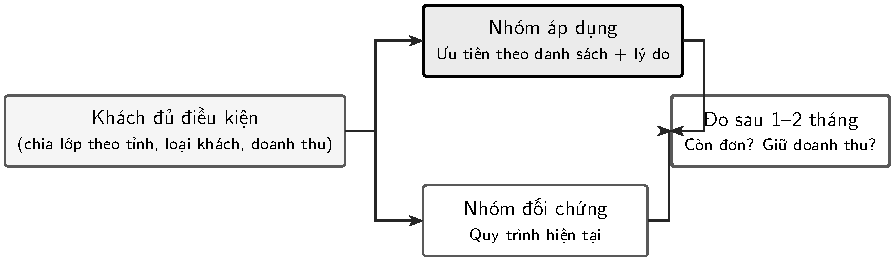
\includegraphics[width=429.4bp]{figures/fig09.pdf}
\caption{Thiết kế thử nghiệm đối chứng}\label{fig:ab}
\end{figure}

{\tablefont
\begin{longtable}{@{}>{\bfseries}L{3.6cm}>{\raggedright\arraybackslash}p{12.03cm}@{}}
\caption{Thiết kế thử nghiệm đề xuất}\label{tab:ab}\\
\toprule
\hdrrow\hh{Hạng mục} & \hh{Thiết kế đề xuất}\\
\midrule
\endfirsthead
\toprule
\hdrrow\hh{Hạng mục} & \hh{Thiết kế đề xuất}\\
\midrule
\endhead
\bottomrule
\endfoot
Đơn vị chia nhóm & Ưu tiên chia ngẫu nhiên ở cấp khách hàng. Nếu khó thực hiện, chia theo tỉnh/nhóm tuyến hoặc triển khai lần lượt theo đợt.\\
\rowa Nhóm áp dụng & Đội chăm sóc ưu tiên khách trong danh sách top 5\% và hành động theo lý do rủi ro.\\
Nhóm đối chứng & Quy trình hiện tại hoặc không dùng điểm rủi ro.\\
\rowa Chọn mẫu & Chỉ lấy khách đủ điều kiện; chia lớp theo tỉnh, loại khách, nhóm doanh thu, nhóm gắn bó để hai nhóm cân bằng.\\
Can thiệp & Chuẩn hóa kịch bản chăm sóc theo từng lý do: giảm đơn, giảm doanh thu, khiếu nại, giao muộn, thu hộ, biến động dịch vụ, hài lòng thấp.\\
\rowa Thời gian đo & Tháng kế tiếp và tháng kế tiếp nữa: còn phát sinh đơn không; số đơn, doanh thu giữ lại; tỷ lệ phản hồi; chi phí chăm sóc mỗi khách giữ được.\\
Rào chắn an toàn & Không làm tăng khiếu nại; không vượt tải của đội chăm sóc; không giảm chất lượng phục vụ nhóm đối chứng; không dùng dữ liệu sai mục đích.\\
\rowa Cách phân tích & Phân tích theo nhóm được chia ban đầu (kể cả khách không phản hồi). Khi không chia ngẫu nhiên hoàn toàn, dùng phương pháp so sánh trước--sau có đối chứng hoặc ghép cặp để giảm sai lệch.\\
\end{longtable}}
\vspace{4pt}

\section{Cơ chế báo cáo và rà soát}

\begin{itemize}
  \item \textbf{Hằng tuần:} nhóm tác giả xem bảng giám sát (chạy thành công, độ lệch dữ liệu, điểm số).
  \item \textbf{Hằng tháng:} báo cáo chỉ tiêu mô hình và vận hành cho đơn vị chăm sóc khách hàng.
  \item \textbf{Cuối đợt thử nghiệm:} báo cáo hiệu quả kinh doanh của đợt thử nghiệm.
\end{itemize}
